\documentclass{standalone}
\usepackage{tikz}
\usepackage{ctex,siunitx}
\setCJKmainfont{Noto Serif CJK SC}
\usepackage{tkz-euclide}
\usepackage{amsmath}
\usetikzlibrary{patterns, calc}
\usetikzlibrary {decorations.pathmorphing, decorations.pathreplacing, decorations.shapes,}
\begin{document}
\small
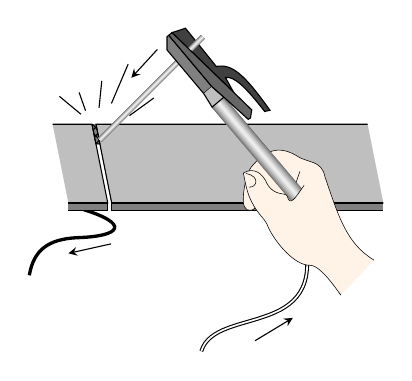
\begin{tikzpicture}[>=latex,scale=1.0]
  % \useasboundingbox(-2,-2.2)rectangle(2,1.5);
  \draw[very thick]( 0.343,-1.069)..controls( 1.013,-1.268)and( 0.865,-1.424)..
  ( 0.311,-1.441)..controls(-0.050,-1.459)and(-0.242,-1.593)..(-0.296,-1.919);
  \draw[double]( 3.137,-1.265)..controls( 3.629,-2.782)and( 2.068,-2.276)..( 1.888,-2.883);
  \draw[-stealth](0.74,-1.52)--(0.2,-1.64);
  \draw[-stealth](2.57,-2.75)--(3.05,-2.46);
  \draw[-stealth](1.33,0.95)--(1,0.59);
  \draw[fill=lightgray] (4,0)--(0.55,0)--(0.75,-1)--(4.2,-1);
  \draw[fill=lightgray] (0,0)--(0.5,0)--(0.7,-1)--(0.2,-1);
  \draw[fill=gray](0.2,-1)--(0.7,-1)--(0.7,-1.1)--(0.2,-1.1);
  \draw[fill=gray](4.2,-1)--(0.75,-1)--(0.75,-1.1)--(4.2,-1.1);
  \draw[fill=gray](0.5,0)--(0.55,-0.25)--(0.6,-0.25)--(0.55,0);
  \draw[pattern = crosshatch,very thin](0.5,0)--(0.55,-0.25)--(0.6,-0.25)--(0.55,0);
  \fill[pink!10!orange!10,draw=black,very thin](3.66,-2.17)--(3.37,-1.72)--(2.628,-0.997)..controls(2.557,-1.102)and(2.483,-1.132)..
  (2.434,-1.043)..controls(2.397,-0.984)and(2.442,-0.644)..
  (2.522,-0.544)..controls(2.617,-0.439)and(2.794,-0.214)..
  (3.099,-0.401)..controls(3.235,-0.496)and(3.417,-0.453)..
  (3.457,-0.664)..controls(3.634,-1.181)and(3.734,-1.517)..(4.083,-1.727);
  \draw[very thin](3.14,-0.60)--(3.06,-0.83);
  \draw[fill=darkgray](2.194,0.594)..controls(2.310,0.609)and(2.446,0.476)..(2.693,0.162)--(2.760,0.177)..controls(2.435,0.632)and(2.280,0.771)..(2.079,0.733)--(1.687,1.219)--(1.516,1.163)--(2.298,0.406)--cycle;
  
  % \draw[fill=darkgray](2.079,0.733)--(1.687,1.219)--(1.516,1.163)--(2.298,0.406)--(2.529,0.181)--(2.512,0.079)--(2.484,0.062)--(2.170,0.339);
  \foreach \w in {80,70,...,10}
  {
    \draw[line width={2*sin(\w)},darkgray!\w](0.6,-0.2)--++(45:1.85);
    \draw[line width={6*sin(\w)},darkgray!\w](3.15,-0.96)--(2.10,0.28);
  }
  \fill[pink!10!orange!10,draw=black,very thin](3.193,-0.776)..controls(3.068,-0.960)and(3.014,-1.039)..
  (2.980,-0.916)..controls(2.969,-0.859)and(2.811,-0.926)..
  (2.720,-0.748)..controls(2.664,-0.623)and(2.556,-0.541)..
  (2.422,-0.620)..controls(2.467,-0.850)and(2.483,-0.909)..
  (2.558,-1.042)..controls(2.635,-1.168)and(2.679,-1.188)..
  (2.721,-1.267)..controls(2.783,-1.443)and(3.053,-1.796)..
  (3.266,-1.791)..controls(3.350,-1.791)and(3.468,-1.896)..(3.659,-2.170);
  \draw[very thin](2.455,-0.626)..controls(2.645,-0.663)and(2.589,-0.810)..(2.494,-0.799);
  \draw[fill=gray](1.475,1.129)--(2.023,0.477)--(1.919,0.389)--(1.453,0.943)--(1.453,1.111)--cycle;
  \draw[fill=lightgray](2.023,0.477)--(2.175,0.343)--(2.025,0.217)--(1.919,0.389);
  \draw[fill=darkgray!80](2.175,0.343)--(2.023,0.477)--(1.475,1.129)--(1.516,1.163)--(2.298,0.406)--(2.529,0.181)--(2.512,0.079)--(2.484,0.062)--cycle;
  \foreach \x/\y/\z/\w in {0.086/0.354/0.359/0.127,0.336/0.404/0.418/0.172,0.624/0.550/0.589/0.207,0.959/0.763/0.746/0.263,1.285/0.333/0.976/0.109}
  {
    \draw(\x,\y)--(\z,\w);
  }
  \end{tikzpicture}
\end{document}